\section{Algoritmo base}
La ejecución de un algoritmo genético se compone de varias fases, en cada una de las cuales se pueden aplicar operadores y algoritmos diferentes que, mezclados con los distintos parámetros que se pueden usar, hacen que estos algoritmos sean muy diversos. Al final, todos los algoritmos genéticos siguen la siguiente estructura:

\begin{figure}[H]
\centering
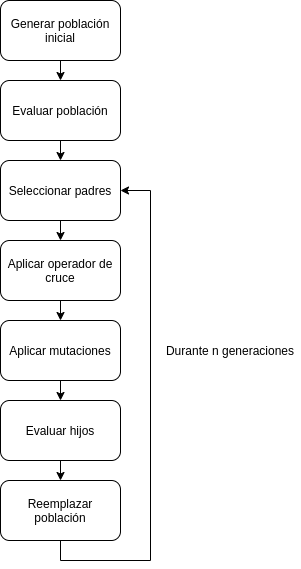
\includegraphics[height=9cm]{images/executionFlow.png}
\end{figure}

Exceptuando la evaluación de los individuos de la población, que se realiza aplicando la función 1 vista en la sección anterior, vamos a ir explicando la implementación escogida para cada una de las partes.

\subsection{Generación de la población inicial}
He decidido usar una población de 100 individuos para el algoritmo, la cuál debe ser inicializada de manera aleatoria. Existen muchas maneras de generar permutaciones aleatorias, de los cuales he decidido aplicar el \textit{Knuth shuffle}. Este algoritmo comienza con una permutación base y va generando nuevas permutaciones cambiando de lugar dos elementos aleatorios de ésta.

\subsection{Selección de los padres}
Del total de la población, debemos elegir un conjunto de individuos para que sean los padres de la nueva generación. Una de las muchas maneras de conseguir esto es mediante torneos, que es el método usado en mi algoritmo. En la selección por torneo, se elige un número $k$ de candidatos aleatorios de la población y se enfrentan unos con otros obteniendo unos ganadores. En mi caso, selecciono 10 candidatos aleatorios de la población inicial y los enfrento de forma determinista para obtener un ganador, es decir, el ganador es el individuo con menor valor de la función de coste.

Repito este procedimiento 100 veces para obtener los 100 padres (los cuales pueden estar repetidos) con los que obtendré los hijos.

\subsection{Cruce de los padres}
Aunque existen muchos operadores de cruce, no todos ellos se pueden aplicar a permutaciones. Los operadores de cruce para representaciones de este tipo deben respetar las restricciones de las mismas. El operador que he aplicado en mi algoritmo es el de cruce de orden, también conocido como \textit{OX}.

Consiste en seleccionar dos índices aleatorios de la permutación que actúa como primer padre y copiar directamente la cadena de elementos que se encuentra entre estos índices a la misma posición en el hijo. A continuación, se rellenan las posiciones que faltan del hijo con los valores del segundo padre que no se encuentran en la cadena copiada, manteniendo el orden de aparición a partir del final de la misma. Dos permutaciones se reparten los roles de primer y segundo padre, obteniendo así 2 hijos.

La probabilidad de cruce es del 100\% lo que significa que todos los padres van a cruzarse. En total, obtenemos 100 nuevos hijos después de cruzar los padres.

\subsection{Mutación de los hijos}
Una vez tenemos los hijos, debemos aplicar un operador de mutación que aporte al algoritmo mayor variabilidad. Cada hijo resultante del cruce de padres tendrá una probabilidad del 80\% de que se le aplique este operador. En mi algoritmo, se usa el intercambio aleatorio como operador de mutación.

Como su propio nombre indica, consiste en seleccionar dos índices aleatorios de la permutación e intercambiar sus elementos de sitio. Los individuos mutados podrán ser mejores o peores que los originales.

\subsection{Reemplazo de la población}
Una vez hemos obtenido y mutado los hijos, debemos incorporar los nuevos individuos a la población actual. Existen varias estrategias para realizar esto (reemplazar la población completa, reemplazar el último elemento, ...), de las que yo he elegido una estrategia elitista.

En el reemplazo elitista, se mantienen los mejores individuos de la generación anterior y se sustituye el resto por los mejores de la nueva generación. En mi caso, me quedo con los 10 mejores individuos y los 90 mejores hijos.